% GNUPLOT: LaTeX picture with Postscript
\begingroup
  \makeatletter
  \providecommand\color[2][]{%
    \GenericError{(gnuplot) \space\space\space\@spaces}{%
      Package color not loaded in conjunction with
      terminal option `colourtext'%
    }{See the gnuplot documentation for explanation.%
    }{Either use 'blacktext' in gnuplot or load the package
      color.sty in LaTeX.}%
    \renewcommand\color[2][]{}%
  }%
  \providecommand\includegraphics[2][]{%
    \GenericError{(gnuplot) \space\space\space\@spaces}{%
      Package graphicx or graphics not loaded%
    }{See the gnuplot documentation for explanation.%
    }{The gnuplot epslatex terminal needs graphicx.sty or graphics.sty.}%
    \renewcommand\includegraphics[2][]{}%
  }%
  \providecommand\rotatebox[2]{#2}%
  \@ifundefined{ifGPcolor}{%
    \newif\ifGPcolor
    \GPcolortrue
  }{}%
  \@ifundefined{ifGPblacktext}{%
    \newif\ifGPblacktext
    \GPblacktexttrue
  }{}%
  % define a \g@addto@macro without @ in the name:
  \let\gplgaddtomacro\g@addto@macro
  % define empty templates for all commands taking text:
  \gdef\gplbacktext{}%
  \gdef\gplfronttext{}%
  \makeatother
  \ifGPblacktext
    % no textcolor at all
    \def\colorrgb#1{}%
    \def\colorgray#1{}%
  \else
    % gray or color?
    \ifGPcolor
      \def\colorrgb#1{\color[rgb]{#1}}%
      \def\colorgray#1{\color[gray]{#1}}%
      \expandafter\def\csname LTw\endcsname{\color{white}}%
      \expandafter\def\csname LTb\endcsname{\color{black}}%
      \expandafter\def\csname LTa\endcsname{\color{black}}%
      \expandafter\def\csname LT0\endcsname{\color[rgb]{1,0,0}}%
      \expandafter\def\csname LT1\endcsname{\color[rgb]{0,1,0}}%
      \expandafter\def\csname LT2\endcsname{\color[rgb]{0,0,1}}%
      \expandafter\def\csname LT3\endcsname{\color[rgb]{1,0,1}}%
      \expandafter\def\csname LT4\endcsname{\color[rgb]{0,1,1}}%
      \expandafter\def\csname LT5\endcsname{\color[rgb]{1,1,0}}%
      \expandafter\def\csname LT6\endcsname{\color[rgb]{0,0,0}}%
      \expandafter\def\csname LT7\endcsname{\color[rgb]{1,0.3,0}}%
      \expandafter\def\csname LT8\endcsname{\color[rgb]{0.5,0.5,0.5}}%
    \else
      % gray
      \def\colorrgb#1{\color{black}}%
      \def\colorgray#1{\color[gray]{#1}}%
      \expandafter\def\csname LTw\endcsname{\color{white}}%
      \expandafter\def\csname LTb\endcsname{\color{black}}%
      \expandafter\def\csname LTa\endcsname{\color{black}}%
      \expandafter\def\csname LT0\endcsname{\color{black}}%
      \expandafter\def\csname LT1\endcsname{\color{black}}%
      \expandafter\def\csname LT2\endcsname{\color{black}}%
      \expandafter\def\csname LT3\endcsname{\color{black}}%
      \expandafter\def\csname LT4\endcsname{\color{black}}%
      \expandafter\def\csname LT5\endcsname{\color{black}}%
      \expandafter\def\csname LT6\endcsname{\color{black}}%
      \expandafter\def\csname LT7\endcsname{\color{black}}%
      \expandafter\def\csname LT8\endcsname{\color{black}}%
    \fi
  \fi
    \setlength{\unitlength}{0.0500bp}%
    \ifx\gptboxheight\undefined%
      \newlength{\gptboxheight}%
      \newlength{\gptboxwidth}%
      \newsavebox{\gptboxtext}%
    \fi%
    \setlength{\fboxrule}{0.5pt}%
    \setlength{\fboxsep}{1pt}%
\begin{picture}(6800.00,4520.00)%
    \gplgaddtomacro\gplbacktext{%
      \csname LTb\endcsname%%
      \put(645,595){\makebox(0,0)[r]{\strut{}$-60$}}%
      \csname LTb\endcsname%%
      \put(645,1062){\makebox(0,0)[r]{\strut{}$-55$}}%
      \csname LTb\endcsname%%
      \put(645,1530){\makebox(0,0)[r]{\strut{}$-50$}}%
      \csname LTb\endcsname%%
      \put(645,1997){\makebox(0,0)[r]{\strut{}$-45$}}%
      \csname LTb\endcsname%%
      \put(645,2464){\makebox(0,0)[r]{\strut{}$-40$}}%
      \csname LTb\endcsname%%
      \put(645,2931){\makebox(0,0)[r]{\strut{}$-35$}}%
      \csname LTb\endcsname%%
      \put(645,3399){\makebox(0,0)[r]{\strut{}$-30$}}%
      \csname LTb\endcsname%%
      \put(645,3866){\makebox(0,0)[r]{\strut{}$-25$}}%
      \csname LTb\endcsname%%
      \put(645,4333){\makebox(0,0)[r]{\strut{}$-20$}}%
      \csname LTb\endcsname%%
      \put(747,409){\makebox(0,0){\strut{}$1$}}%
      \csname LTb\endcsname%%
      \put(1568,409){\makebox(0,0){\strut{}$3$}}%
      \csname LTb\endcsname%%
      \put(2389,409){\makebox(0,0){\strut{}$5$}}%
      \csname LTb\endcsname%%
      \put(3210,409){\makebox(0,0){\strut{}$7$}}%
      \csname LTb\endcsname%%
      \put(4030,409){\makebox(0,0){\strut{}$9$}}%
      \csname LTb\endcsname%%
      \put(4851,409){\makebox(0,0){\strut{}$11$}}%
      \csname LTb\endcsname%%
      \put(5672,409){\makebox(0,0){\strut{}$13$}}%
      \csname LTb\endcsname%%
      \put(6493,409){\makebox(0,0){\strut{}$15$}}%
    }%
    \gplgaddtomacro\gplfronttext{%
      \csname LTb\endcsname%%
      \put(153,2464){\rotatebox{-270}{\makebox(0,0){\strut{}Interaction energy (kcal/mol)}}}%
      \csname LTb\endcsname%%
      \put(3620,130){\makebox(0,0){\strut{}\# units}}%
      \csname LTb\endcsname%%
      \put(5807,3282){\makebox(0,0)[r]{\strut{}RI-SCS-MP2/cc-pVDZ}}%
      \csname LTb\endcsname%%
      \put(5807,3561){\makebox(0,0)[r]{\strut{}RI-SCS-MP2/cc-pVTZ}}%
      \csname LTb\endcsname%%
      \put(5807,3840){\makebox(0,0)[r]{\strut{}DLPNO-CCSD(T)/cc-pVDZ}}%
      \csname LTb\endcsname%%
      \put(5807,4119){\makebox(0,0)[r]{\strut{}approximate DLPNO-CCSD(T)/cc-pVTZ}}%
    }%
    \gplbacktext
    \put(0,0){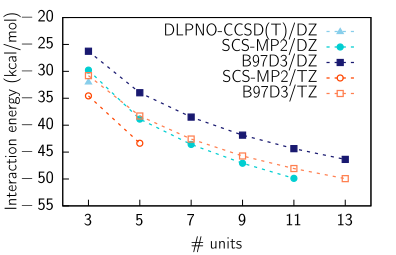
\includegraphics{n3_t55x_eint}}%
    \gplfronttext
  \end{picture}%
\endgroup
